% Options for packages loaded elsewhere
\PassOptionsToPackage{unicode}{hyperref}
\PassOptionsToPackage{hyphens}{url}
\PassOptionsToPackage{dvipsnames,svgnames,x11names}{xcolor}
%
\documentclass[
  ignorenonframetext,
  aspectratio=169,
]{beamer}
\usepackage{pgfpages}
\setbeamertemplate{caption}[numbered]
\setbeamertemplate{caption label separator}{: }
\setbeamercolor{caption name}{fg=normal text.fg}
\beamertemplatenavigationsymbolshorizontal
% Prevent slide breaks in the middle of a paragraph
\widowpenalties 1 10000
\raggedbottom
\setbeamertemplate{part page}{
  \centering
  \begin{beamercolorbox}[sep=16pt,center]{part title}
    \usebeamerfont{part title}\insertpart\par
  \end{beamercolorbox}
}
\setbeamertemplate{section page}{
  \centering
  \begin{beamercolorbox}[sep=12pt,center]{part title}
    \usebeamerfont{section title}\insertsection\par
  \end{beamercolorbox}
}
\setbeamertemplate{subsection page}{
  \centering
  \begin{beamercolorbox}[sep=8pt,center]{part title}
    \usebeamerfont{subsection title}\insertsubsection\par
  \end{beamercolorbox}
}
\AtBeginPart{
  \frame{\partpage}
}
\AtBeginSection{
  \ifbibliography
  \else
    \frame{\sectionpage}
  \fi
}
\AtBeginSubsection{
  \frame{\subsectionpage}
}

\usepackage{amsmath,amssymb}
\usepackage{iftex}
\ifPDFTeX
  \usepackage[T1]{fontenc}
  \usepackage[utf8]{inputenc}
  \usepackage{textcomp} % provide euro and other symbols
\else % if luatex or xetex
  \usepackage{unicode-math}
  \defaultfontfeatures{Scale=MatchLowercase}
  \defaultfontfeatures[\rmfamily]{Ligatures=TeX,Scale=1}
\fi
\usetheme[]{CambridgeUS}
\usecolortheme{orchid}
\usepackage[]{libertinus}
\ifPDFTeX\else  
    % xetex/luatex font selection
\fi
% Use upquote if available, for straight quotes in verbatim environments
\IfFileExists{upquote.sty}{\usepackage{upquote}}{}
\IfFileExists{microtype.sty}{% use microtype if available
  \usepackage[]{microtype}
  \UseMicrotypeSet[protrusion]{basicmath} % disable protrusion for tt fonts
}{}
\makeatletter
\@ifundefined{KOMAClassName}{% if non-KOMA class
  \IfFileExists{parskip.sty}{%
    \usepackage{parskip}
  }{% else
    \setlength{\parindent}{0pt}
    \setlength{\parskip}{6pt plus 2pt minus 1pt}}
}{% if KOMA class
  \KOMAoptions{parskip=half}}
\makeatother
\usepackage{xcolor}
\newif\ifbibliography
\setlength{\emergencystretch}{3em} % prevent overfull lines
\setcounter{secnumdepth}{-\maxdimen} % remove section numbering


\providecommand{\tightlist}{%
  \setlength{\itemsep}{0pt}\setlength{\parskip}{0pt}}\usepackage{longtable,booktabs,array}
\usepackage{calc} % for calculating minipage widths
\usepackage{caption}
% Make caption package work with longtable
\makeatletter
\def\fnum@table{\tablename~\thetable}
\makeatother
\usepackage{graphicx}
\makeatletter
\def\maxwidth{\ifdim\Gin@nat@width>\linewidth\linewidth\else\Gin@nat@width\fi}
\def\maxheight{\ifdim\Gin@nat@height>\textheight\textheight\else\Gin@nat@height\fi}
\makeatother
% Scale images if necessary, so that they will not overflow the page
% margins by default, and it is still possible to overwrite the defaults
% using explicit options in \includegraphics[width, height, ...]{}
\setkeys{Gin}{width=\maxwidth,height=\maxheight,keepaspectratio}
% Set default figure placement to htbp
\makeatletter
\def\fps@figure{htbp}
\makeatother

\input{/Users/joseph/GIT/latex/latex-for-quarto.tex}
\makeatletter
\@ifpackageloaded{caption}{}{\usepackage{caption}}
\AtBeginDocument{%
\ifdefined\contentsname
  \renewcommand*\contentsname{Table of contents}
\else
  \newcommand\contentsname{Table of contents}
\fi
\ifdefined\listfigurename
  \renewcommand*\listfigurename{List of Figures}
\else
  \newcommand\listfigurename{List of Figures}
\fi
\ifdefined\listtablename
  \renewcommand*\listtablename{List of Tables}
\else
  \newcommand\listtablename{List of Tables}
\fi
\ifdefined\figurename
  \renewcommand*\figurename{Figure}
\else
  \newcommand\figurename{Figure}
\fi
\ifdefined\tablename
  \renewcommand*\tablename{Table}
\else
  \newcommand\tablename{Table}
\fi
}
\@ifpackageloaded{float}{}{\usepackage{float}}
\floatstyle{ruled}
\@ifundefined{c@chapter}{\newfloat{codelisting}{h}{lop}}{\newfloat{codelisting}{h}{lop}[chapter]}
\floatname{codelisting}{Listing}
\newcommand*\listoflistings{\listof{codelisting}{List of Listings}}
\makeatother
\makeatletter
\makeatother
\makeatletter
\@ifpackageloaded{caption}{}{\usepackage{caption}}
\@ifpackageloaded{subcaption}{}{\usepackage{subcaption}}
\makeatother
\ifLuaTeX
  \usepackage{selnolig}  % disable illegal ligatures
\fi
\usepackage{bookmark}

\IfFileExists{xurl.sty}{\usepackage{xurl}}{} % add URL line breaks if available
\urlstyle{same} % disable monospaced font for URLs
\hypersetup{
  pdftitle={Causal Inference in Three-Wave Panel Designs},
  pdfauthor={Joseph A. Bulbulia},
  colorlinks=true,
  linkcolor={Maroon},
  filecolor={Maroon},
  citecolor={Blue},
  urlcolor={Blue},
  pdfcreator={LaTeX via pandoc}}

\title{Causal Inference in Three-Wave Panel Designs}
\subtitle{with illustrations from the New Zealand Attitudes and Values
Study}
\author{Joseph A. Bulbulia}
\date{}
\institute{Joseph.Bulbulia@vuw.ac.nz (Victoria University)}

\begin{document}
\frame{\titlepage}

\begin{frame}{The Fundamental Problem of Causal Inference: We Require a
Counterfactual Contrast}
\phantomsection\label{the-fundamental-problem-of-causal-inference-we-require-a-counterfactual-contrast}
\[Y_{\text{you}}(1) - Y_{\text{you}}(0)\]\footnote<.->{\(Y\) denotes the
  outcome; \(A\) denotes a treatment, \(Y(a)\) denotes the outcome when
  \(A=a\)}
\end{frame}

\begin{frame}{But Individuals Experience Only \textbf{One} Treatment}
\phantomsection\label{but-individuals-experience-only-one-treatment}
\[
Y_i|A_i = 1 \implies Y_i(0)|A_i = 1~ \text{is counterfactual}
\]
\end{frame}

\begin{frame}{Average Treatment Effect in Randomised Controlled
Experiments Work From Assumptions}
\phantomsection\label{average-treatment-effect-in-randomised-controlled-experiments-work-from-assumptions}
\[
\text{Average Treatment Effect} = \left[ \begin{aligned}
&\left( \underbrace{\mathbb{E}[Y(1)|A = 1]}_{\text{observed}} + \textcolor{red}{\underbrace{\mathbb{E}[Y(1)|A = 0]}_{\text{unobserved}}} \right) \\
&- \left( \underbrace{\mathbb{E}[Y(0)|A = 0]}_{\text{observed}} + \textcolor{red}{\underbrace{\mathbb{E}[Y(0)|A = 1]}_{\text{unobserved}}} \right)
\end{aligned} \right]
\]
\end{frame}

\section{The Three Fundemental Assumptions of Causal
Inference}\label{the-three-fundemental-assumptions-of-causal-inference}

\begin{frame}{Causal Consistency}
\phantomsection\label{causal-consistency}
\[
Y_i^{observed}|A_i = 
\begin{cases} 
Y_i(a^*) & \text{if } A_i = a^* \\
Y_i(a) & \text{if } A_i = a
\end{cases}
\]
\end{frame}

\begin{frame}{Conditional Exchangeabilty}
\phantomsection\label{conditional-exchangeabilty}
\[
Y(a) \coprod A | L \quad \text{or equivalently} \quad A \coprod Y(a) | L
\]\footnote<.->{\(L\) denotes measured covariates.}
\end{frame}

\begin{frame}{Positivity}
\phantomsection\label{positivity}
\[
0 < Pr(A = a | L = l) < 1
\]
\end{frame}

\begin{frame}{The Typical \textbf{Worry}: Confounding by Common Cause}
\phantomsection\label{the-typical-worry-confounding-by-common-cause}
\[\commoncauseA\]
\end{frame}

\begin{frame}{However, There Are Other \textbf{Worries}: Reverse
Causation}
\phantomsection\label{however-there-are-other-worries-reverse-causation}
\[\ytoa\]
\end{frame}

\begin{frame}{Another \textbf{Worry} is Mediator Bias}
\phantomsection\label{another-worry-is-mediator-bias}
\[\mediatorA\]
\end{frame}

\begin{frame}{Another \textbf{Worry} is Collider Bias}
\phantomsection\label{another-worry-is-collider-bias}
\[\colliderALONG\]
\end{frame}

\begin{frame}{Another \textbf{Worry} is Collider Bias Proxy}
\phantomsection\label{another-worry-is-collider-bias-proxy}
\[\descendantBBLONG\]
\end{frame}

\begin{frame}{Yet Another \textbf{Worry} is Post Exposure Collider Bias}
\phantomsection\label{yet-another-worry-is-post-exposure-collider-bias}
\[\mediatorcollider\]\footnote<.->{\(U\) denotes and unmeasured
  confounder of \(A\to Y\)\}}
\end{frame}

\begin{frame}{Another \textbf{Worry} are Unmeasured Common Causes
(\(U\))}
\phantomsection\label{another-worry-are-unmeasured-common-causes-u}
\[\downstream\]
\end{frame}

\begin{frame}{Reverse Causation Strategy: \textbf{Longitudinal Hygiene}}
\phantomsection\label{reverse-causation-strategy-longitudinal-hygiene}
\begin{columns}[T]
\begin{column}{0.5\textwidth}
\[\ytoa\]
\end{column}

\begin{column}{0.5\textwidth}
\[\aandysolution\]
\end{column}
\end{columns}
\end{frame}

\begin{frame}{Mediator Bias Strategy: \textbf{Longitudinal Hygiene}}
\phantomsection\label{mediator-bias-strategy-longitudinal-hygiene}
\begin{columns}[T]
\begin{column}{0.5\textwidth}
\[
\mediatorA
\]
\end{column}

\begin{column}{0.5\textwidth}
\[
\commoncausesolvedA
\]
\end{column}
\end{columns}
\end{frame}

\begin{frame}{Collider Bias Strategy: \textbf{Longitudinal Hygiene}}
\phantomsection\label{collider-bias-strategy-longitudinal-hygiene}
\begin{columns}[T]
\begin{column}{0.5\textwidth}
\[\colliderALONG\]
\end{column}

\begin{column}{0.5\textwidth}
\[\commoncausesolvedA\]
\end{column}
\end{columns}
\end{frame}

\begin{frame}{Collider Bias Proxy Strategy: \textbf{Longitudinal
Hygiene}}
\phantomsection\label{collider-bias-proxy-strategy-longitudinal-hygiene}
\begin{columns}[T]
\begin{column}{0.5\textwidth}
\[\descendantBBLONG\]
\end{column}

\begin{column}{0.5\textwidth}
\[\commoncausesolvedchild\]
\end{column}
\end{columns}
\end{frame}

\begin{frame}{Post Exposure Collider Bias Strategy:\textbf{Longitudinal
Hygiene}}
\phantomsection\label{post-exposure-collider-bias-strategylongitudinal-hygiene}
\begin{columns}[T]
\begin{column}{0.5\textwidth}
\[\mediatorcollider\]
\end{column}

\begin{column}{0.5\textwidth}
\[\commoncausesolvedA\]
\end{column}
\end{columns}
\end{frame}

\begin{frame}{Unmeasured Common Cause Strategy: \textbf{Longitudinal
Hygiene}}
\phantomsection\label{unmeasured-common-cause-strategy-longitudinal-hygiene}
\begin{columns}[T]
\begin{column}{0.5\textwidth}
\[\downstream\]
\end{column}

\begin{column}{0.5\textwidth}
\[\commoncausesolvedA\]
\end{column}
\end{columns}
\end{frame}

\section{New Zealand Attitudes and Values Study
(NZAVS)}\label{new-zealand-attitudes-and-values-study-nzavs}

\begin{frame}{NZAVS \textbf{Longitudinally Hygienic} Data Collection}
\phantomsection\label{nzavs-longitudinally-hygienic-data-collection}
\begin{itemize}
\item
  Planned 20-year longitudinal study, currently in its 14\(^{th}\) year.
\item
  Sample frame is drawn randomly from NZ Electoral Roll.
\item
  Postal questionnaire (coverage; retention \textasciitilde{} 80\%)
\item
  Large multidisciplinary research team (40 +)
\item
  Focus on personality, social attitudes, values, religion, employment,
  prejudice \(\dots\)
\item
  Current sample contains 72910 unique individuals, and
  \textasciitilde{} 38,000 in the longitudinal study
\end{itemize}
\end{frame}

\begin{frame}
\begin{figure}[H]

{\centering 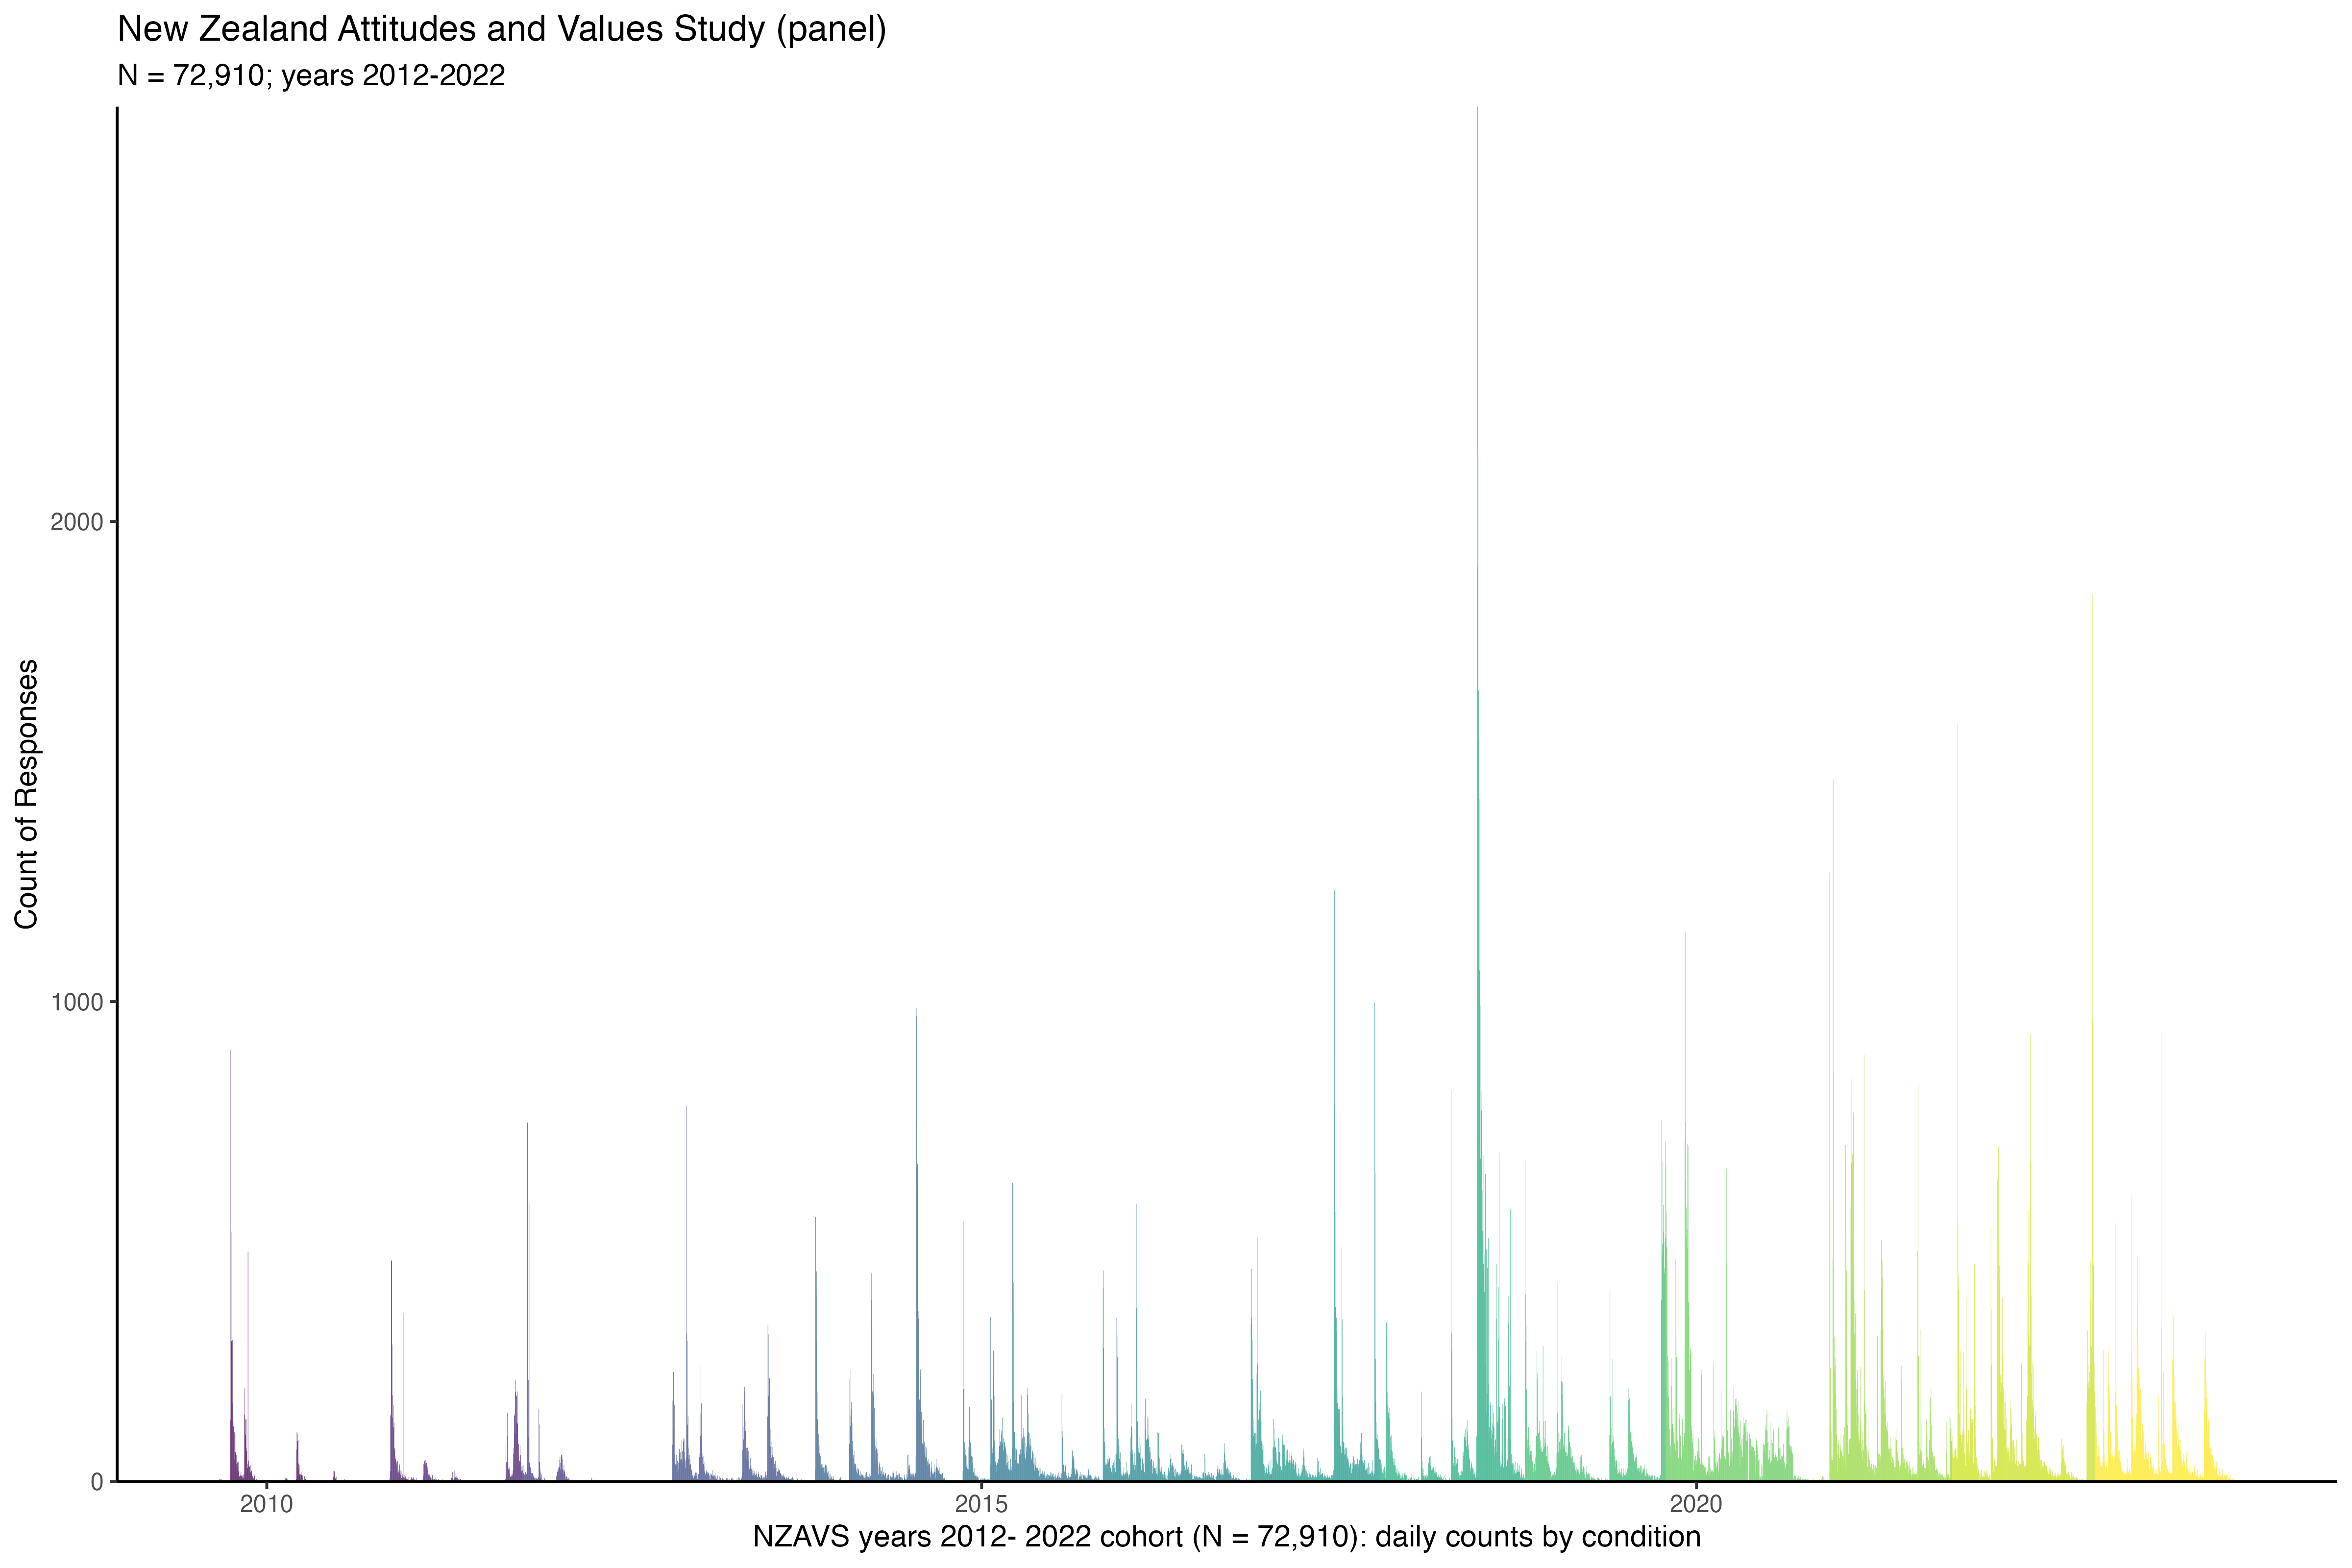
\includegraphics{timeline_histgram_2009_2024.png}

}

\caption{NZAVS Daily Responses}

\end{figure}%
\end{frame}

\begin{frame}
\LARGE \centering BIG EVENTS
\end{frame}

\begin{frame}
\begin{figure}[H]

{\centering \includegraphics{muslim_attack_discontinuity_2012_2022_include_opt_in.png}

}

\caption{Mosque Attacks: Full Sample}

\end{figure}%
\end{frame}

\begin{frame}{Institutional Trust}
\phantomsection\label{institutional-trust}
\textbf{COVID-19 Government response} - ``I trust the Government to make
sensible decisions about how to best manage COVID-19 in New Zealand.'' -
``The New Zealand government response to COVID-19.''

\textbf{Trust in politicians} - ``Politicians in New Zealand can
generally be trusted.''

\textbf{Institutional trust in police} - ``People's basic rights are
well protected by the New Zealand Police.'' - ``There are many things
about the New Zealand Police and its policies that need to be changed.''
- ``The New Zealand Police care about the well-being of everyone they
deal with.''

\textbf{General tendency to believe in conspiracies} - ``I think that
the official version of major world events given by authorities often
hides the truth.''
\end{frame}

\begin{frame}
\begin{figure}[H]

{\centering \includegraphics{plot_rdd_covid_trust_politicians.png}

}

\caption{plot\_rdd\_covid\_trust\_politicians}

\end{figure}%
\end{frame}

\begin{frame}
\begin{figure}[H]

{\centering \includegraphics{plot_rdd_covid_trust_police.png}

}

\caption{plot\_rdd\_covid\_trust\_police}

\end{figure}%
\end{frame}

\begin{frame}
\begin{figure}[H]

{\centering \includegraphics{plot_rdd_covid_trust_science.png}

}

\caption{plot\_rdd\_covid\_trust\_science}

\end{figure}%
\end{frame}

\begin{frame}
\begin{figure}[H]

{\centering \includegraphics{plot_rdd_covid_trust_conspiracy.png}

}

\caption{plot\_rdd\_covid\_trust\_conspiracy}

\end{figure}%
\end{frame}

\begin{frame}{Regulate Gov't Surveillance vs Regulate AI}
\phantomsection\label{regulate-govt-surveillance-vs-regulate-ai}
\end{frame}

\begin{frame}
\begin{figure}[H]

{\centering \includegraphics{better_combo_graph_govt_surveillance_ai.png}

}

\caption{better\_combo\_graph\_govt\_surveillance\_ai}

\end{figure}%
\end{frame}

\begin{frame}
\begin{figure}[H]

{\centering 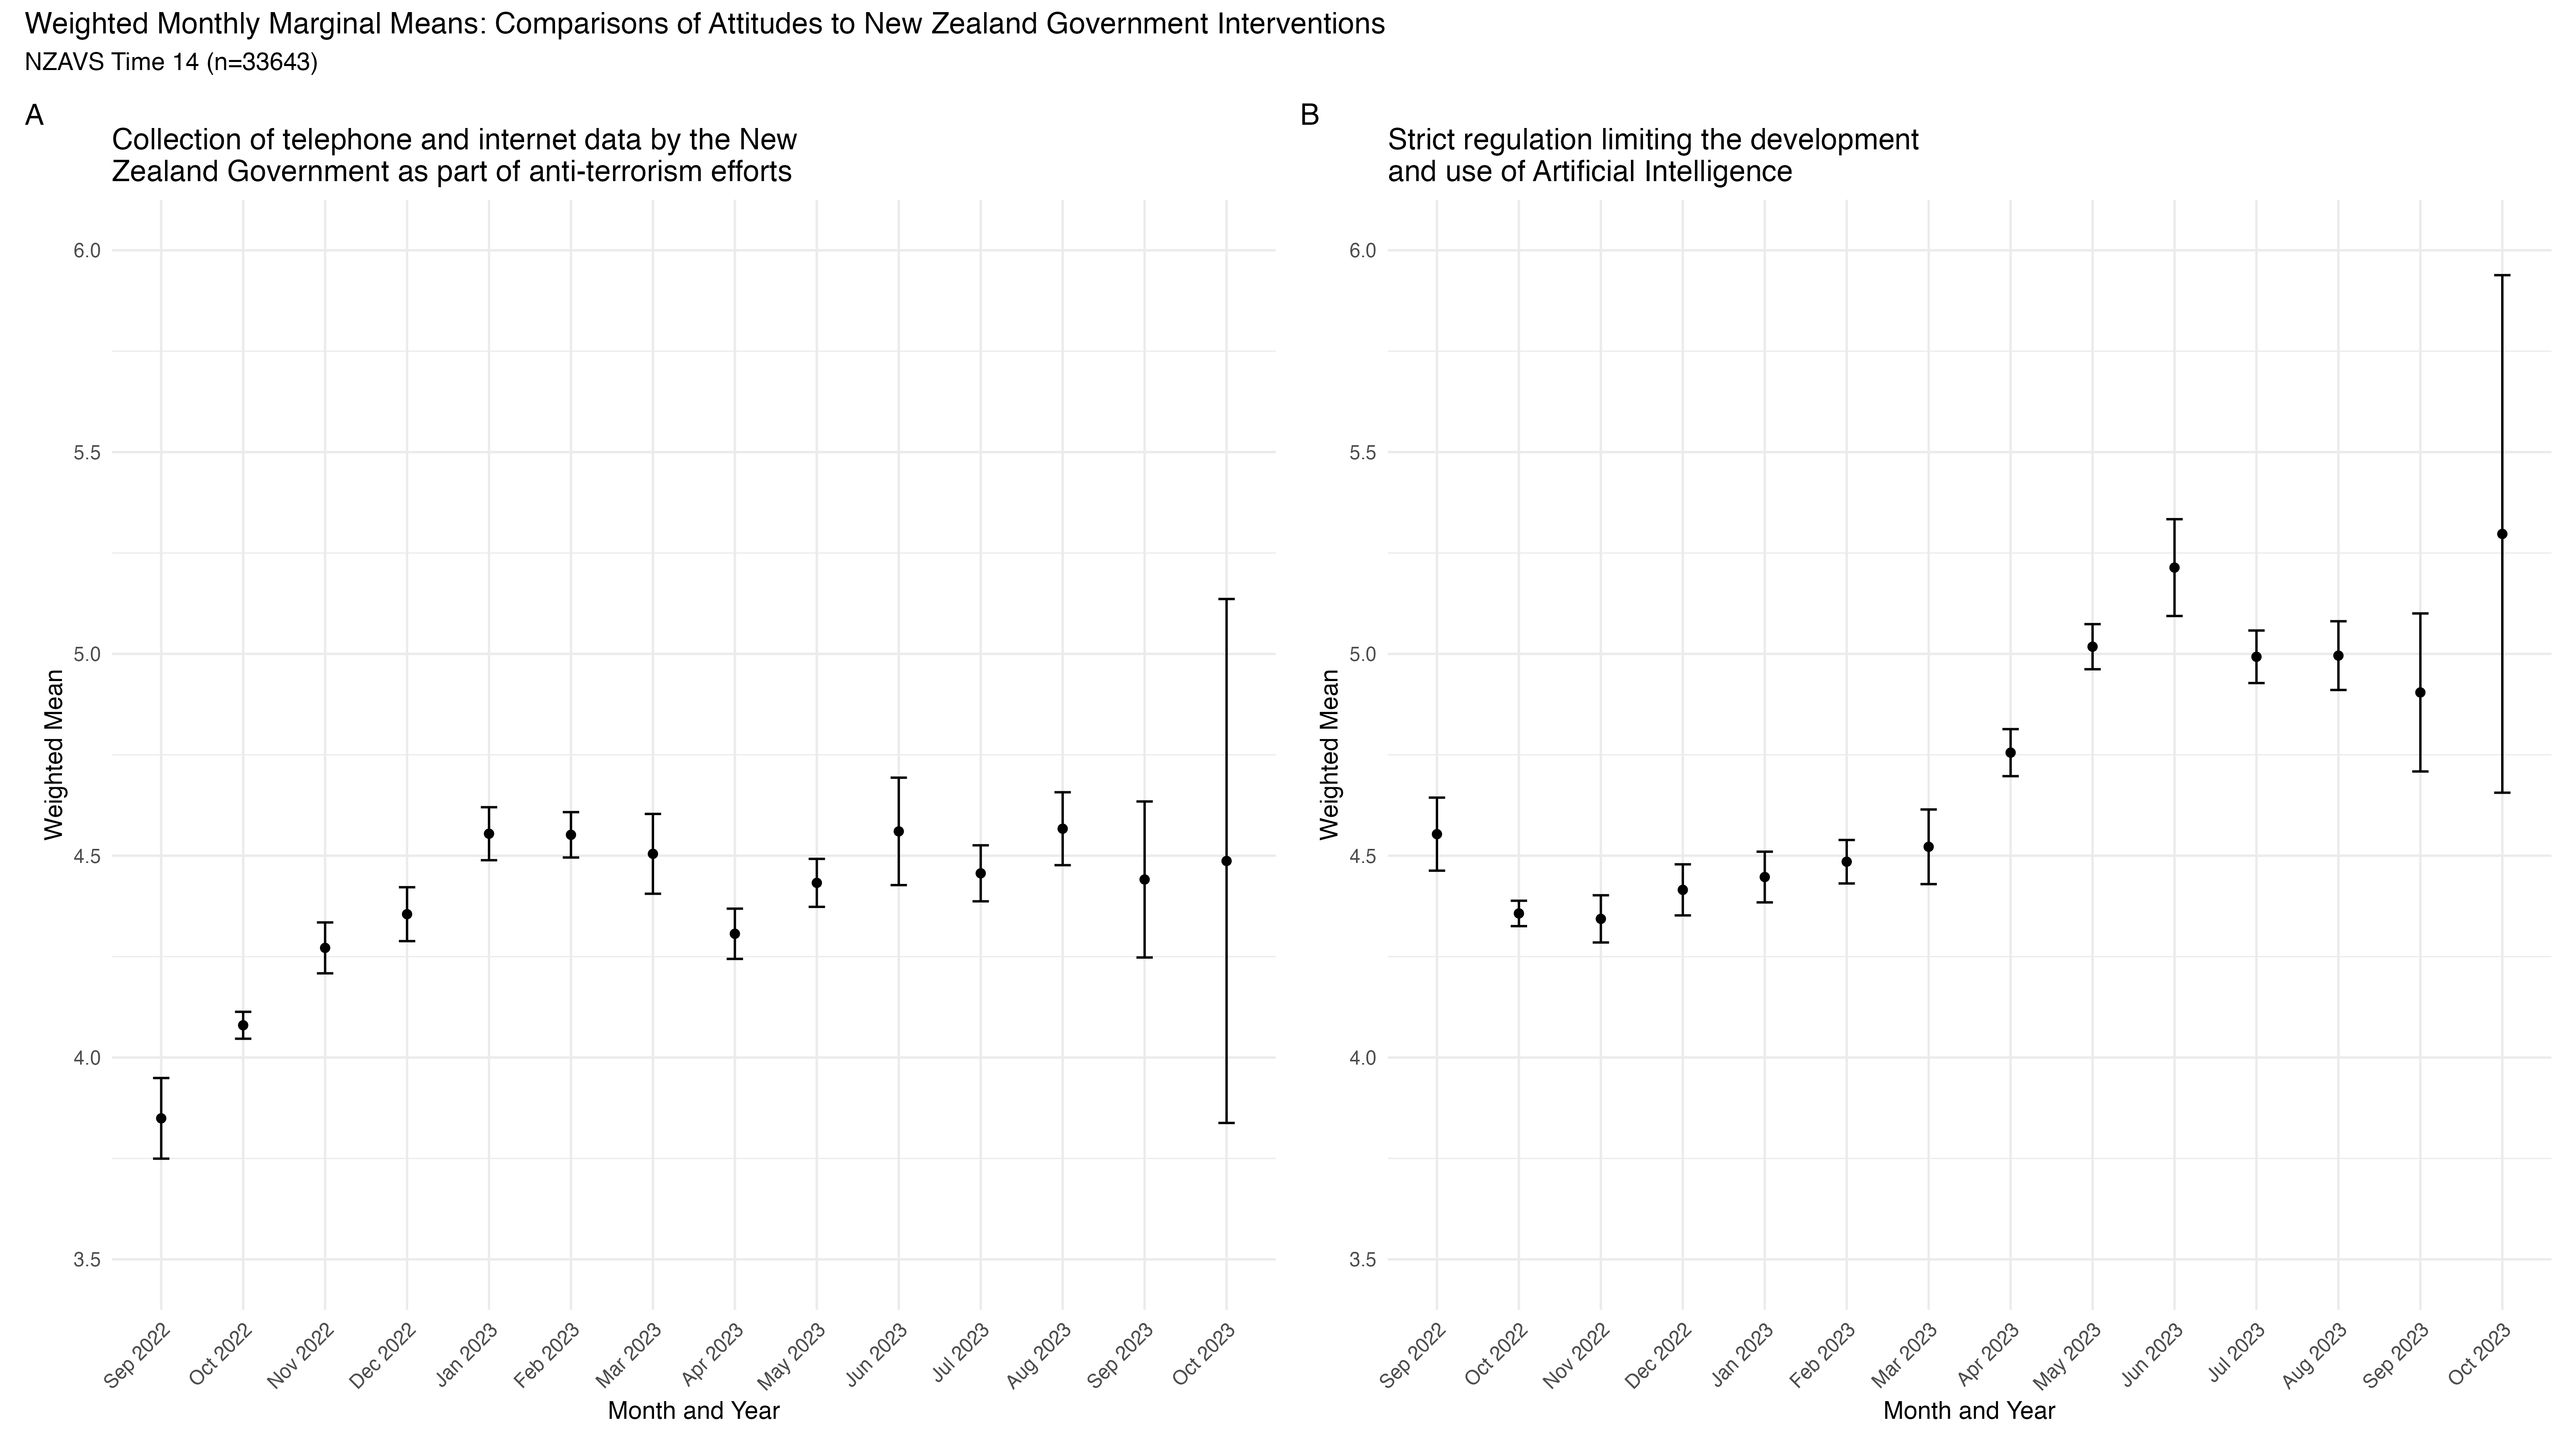
\includegraphics{plot_compare_monthly_weighted_means_govt_surveillance_ai.png}

}

\caption{plot\_compare\_monthly\_weighted\_means\_govt\_surveillance\_ai}

\end{figure}%
\end{frame}

\begin{frame}
\Large \centering Consider Gradual Events
\end{frame}

\begin{frame}
\begin{figure}[H]

{\centering 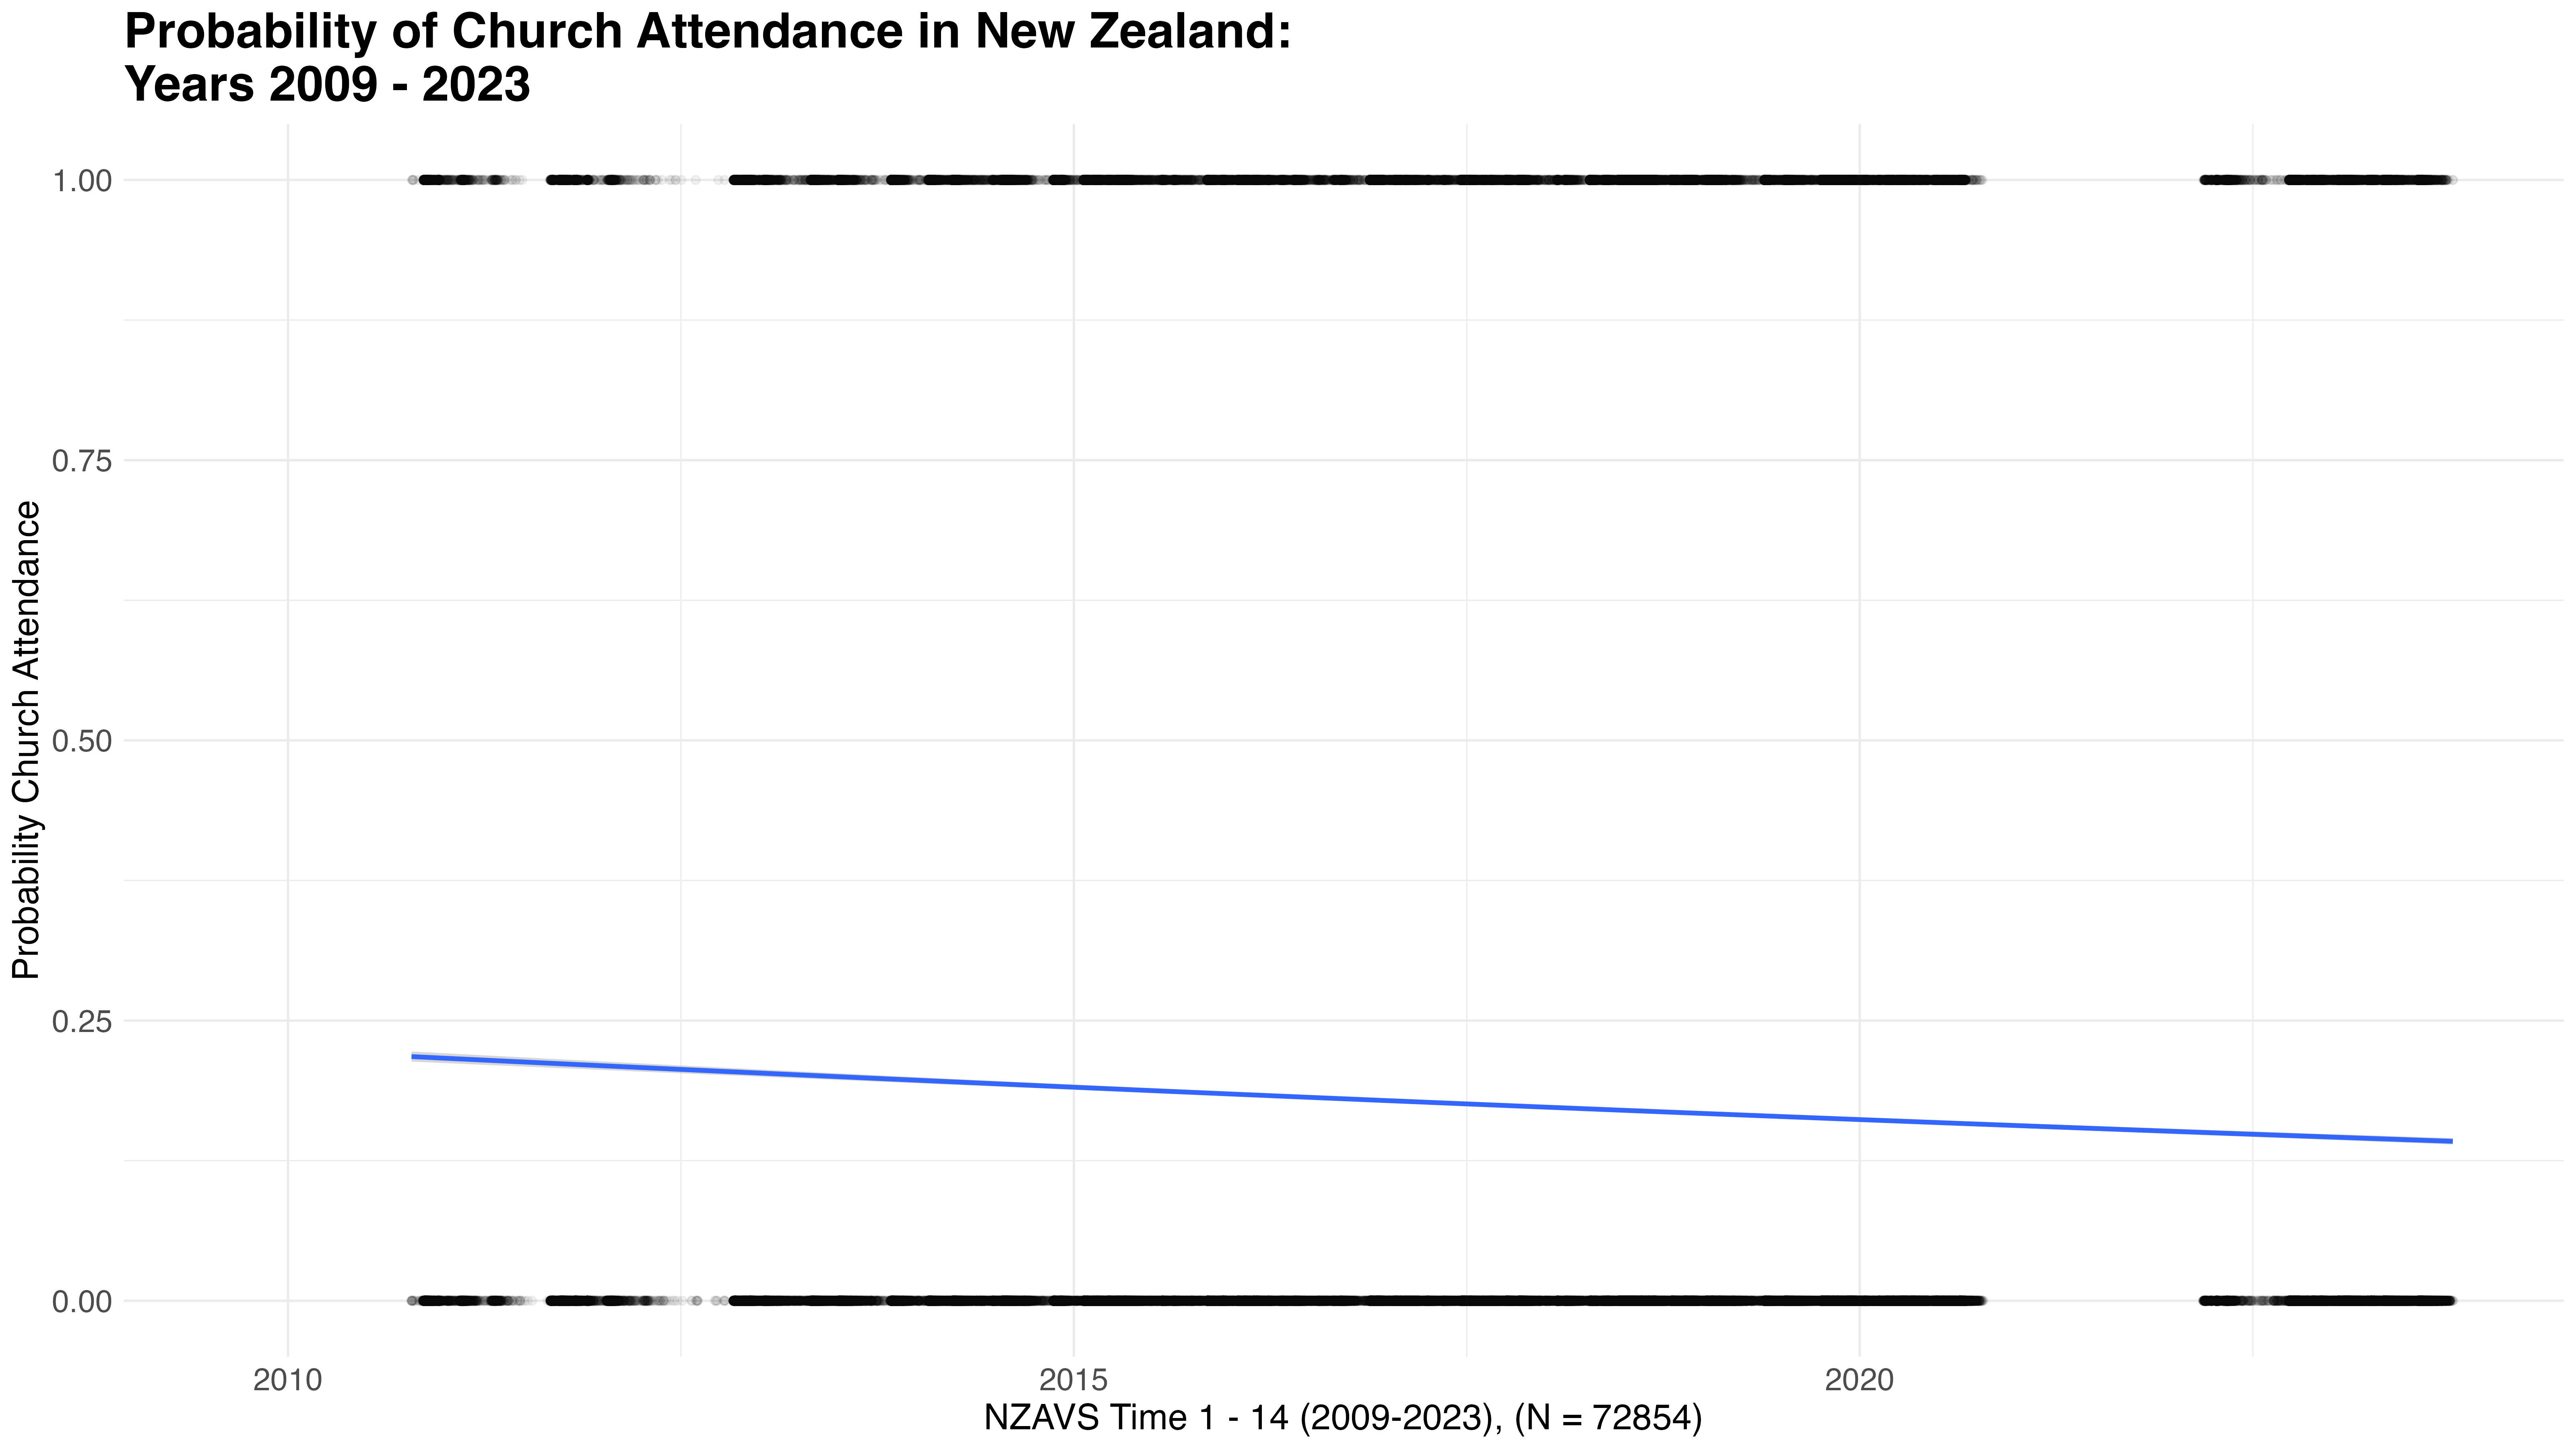
\includegraphics{plot_prob_church_attendance_nz_2009to2024.png}

}

\caption{plot\_prob\_church\_attendance\_nz\_2009to2024}

\end{figure}%
\end{frame}

\begin{frame}{Worked Example: causal Effects of Religious Service on
Prosociality}
\phantomsection\label{worked-example-causal-effects-of-religious-service-on-prosociality}
\begin{block}{Intervention}
\phantomsection\label{intervention}
\[f(A = a*) = \begin{cases} 4 & \text{if } A < 4  \text{ monthly religious service attendance} \\ \tilde{A} & \text{if } A \geq 4  \text{ monthly religious service attendance} \end{cases} \]
\end{block}

\begin{block}{Contrast}
\phantomsection\label{contrast}
\[f(A) = 0 \]
\end{block}
\end{frame}

\begin{frame}{Shift Intervention: Socializing}
\phantomsection\label{shift-intervention-socializing}
\begin{block}{Intervention}
\phantomsection\label{intervention-1}
\[f(A) = \begin{cases} 1.4 & \text{if } A \leq 1.4 \text{ hours socialising with community} \\ \tilde{A} & \text{if } A >  1.4  \text{ hours socialising with community}  \end{cases} \]
\end{block}

\begin{block}{Contrast:}
\phantomsection\label{contrast-1}
\[f(A) = 0 \]
\end{block}
\end{frame}

\begin{frame}{\textbf{Key Graph}}
\phantomsection\label{key-graph}
\[
\threeLONG
\]
\end{frame}

\begin{frame}{Religious Service Outcomes}
\phantomsection\label{religious-service-outcomes}
\end{frame}

\begin{frame}
\begin{figure}[H]

{\centering 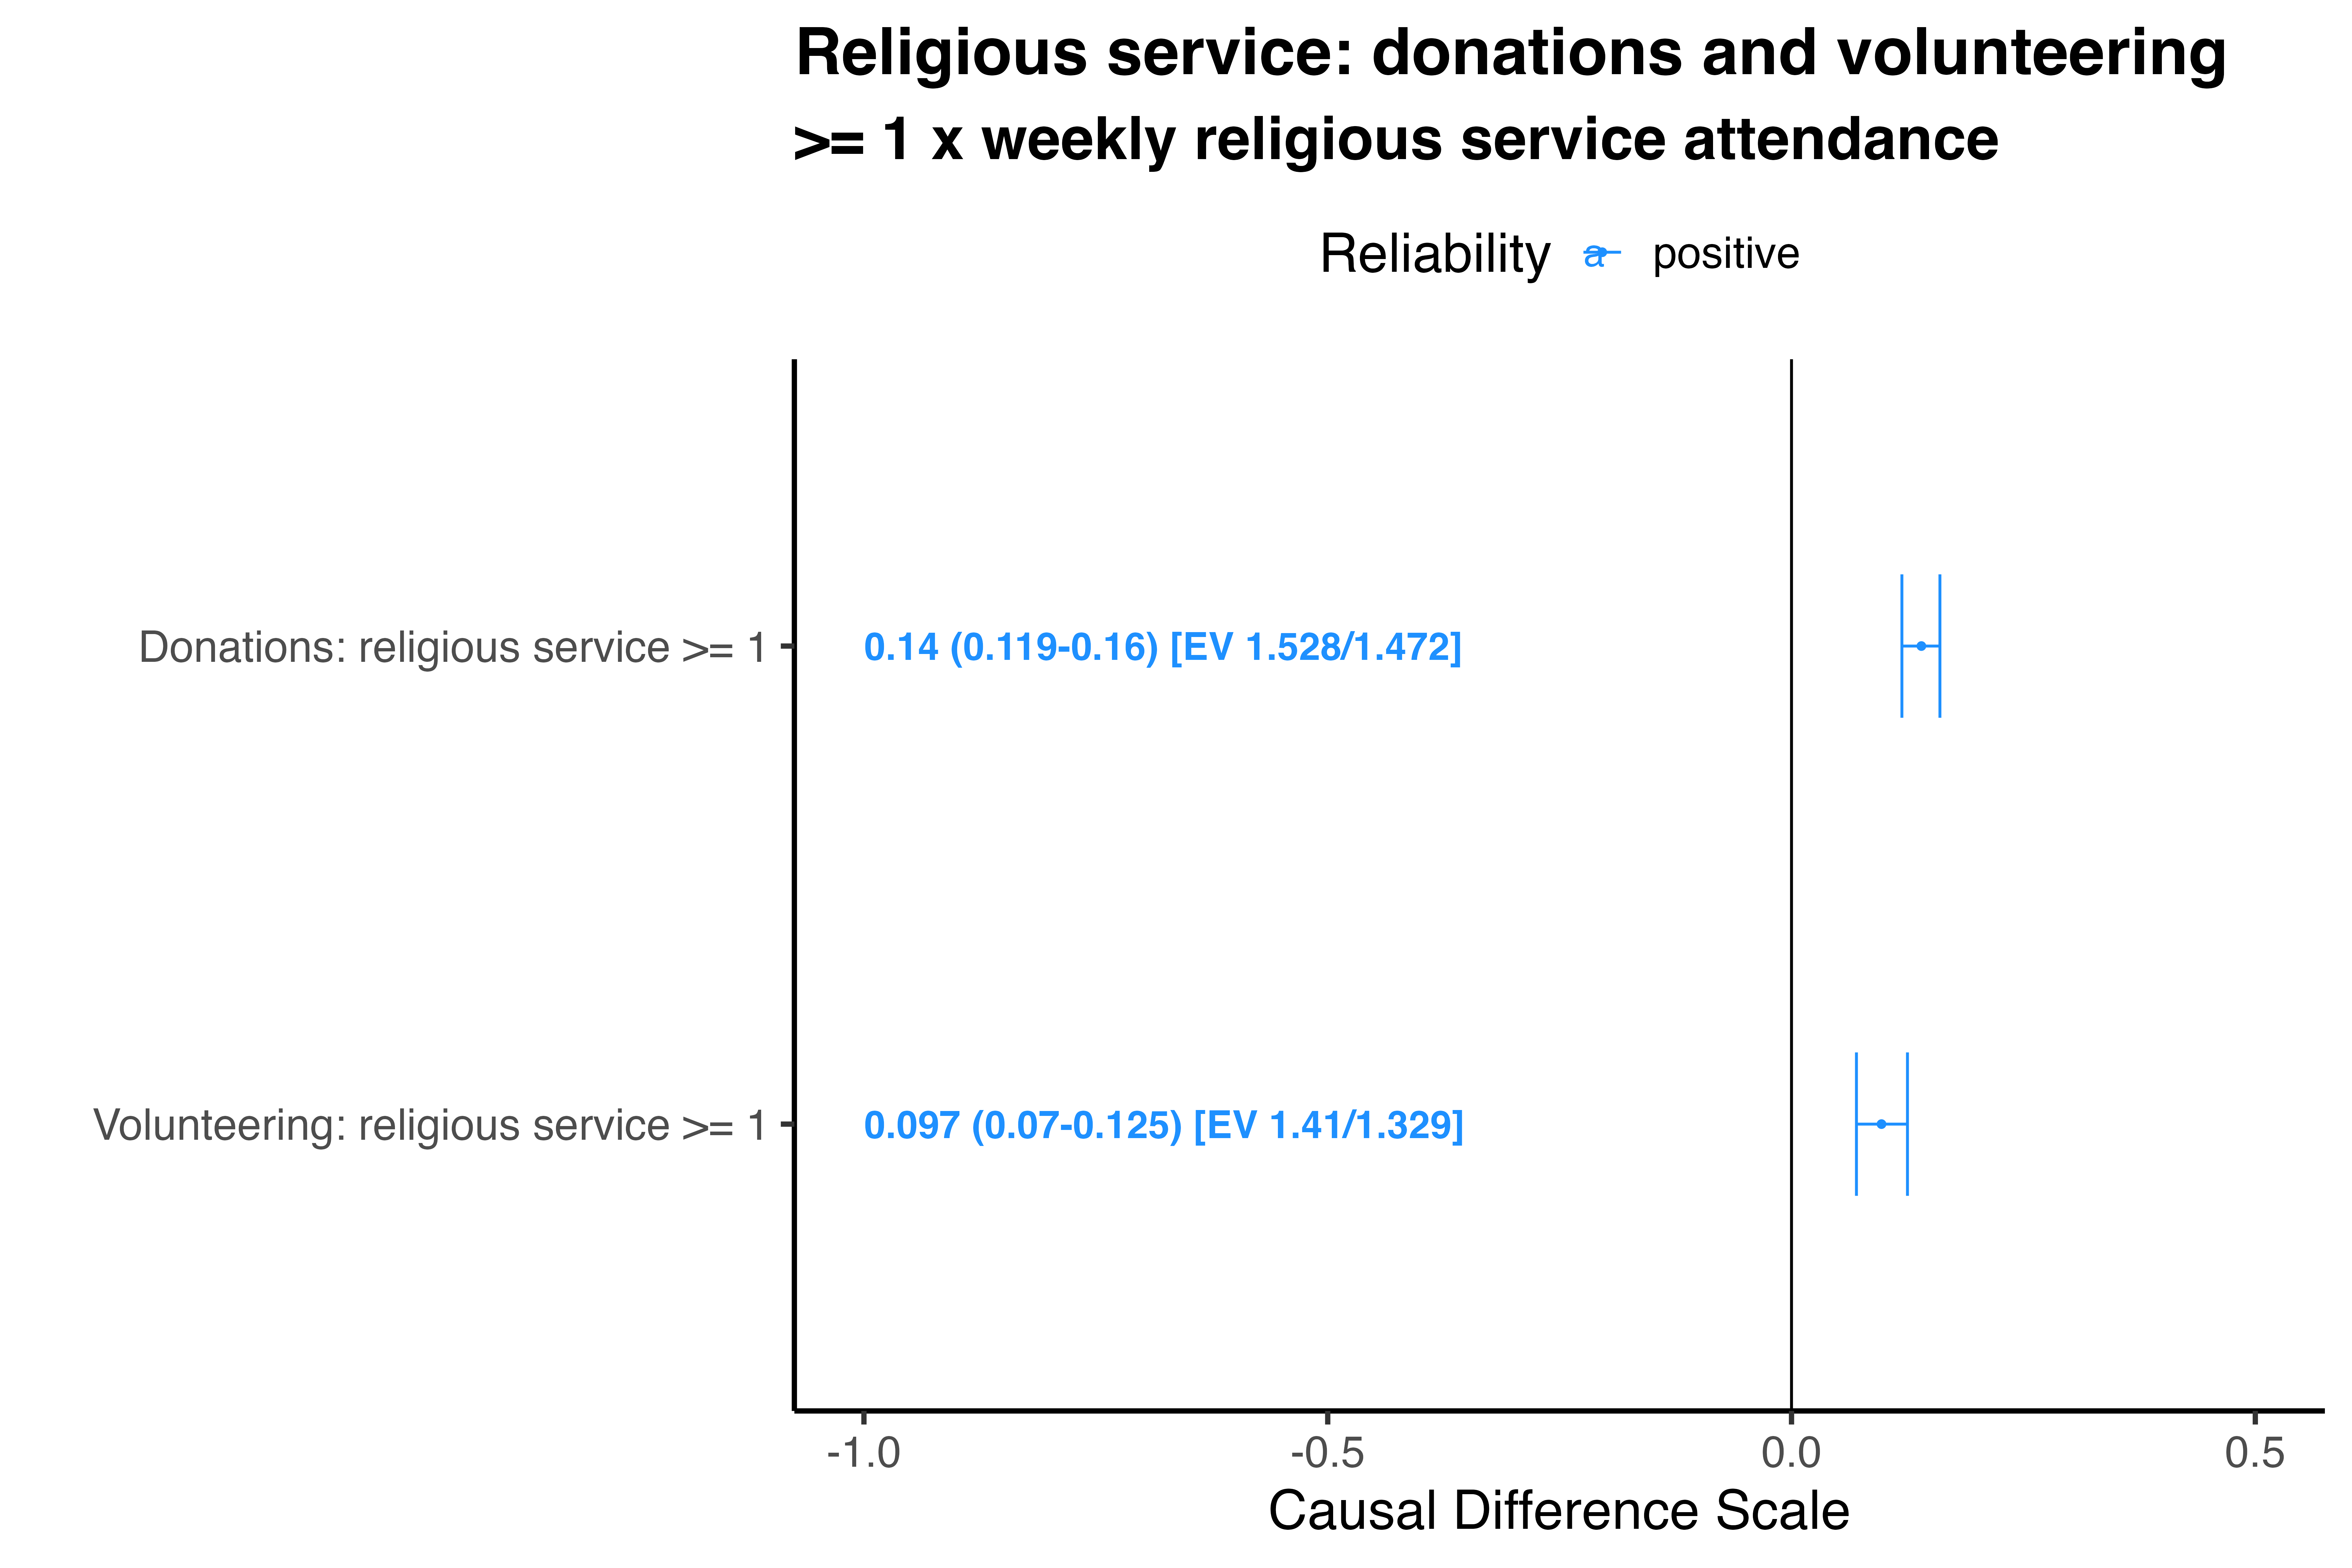
\includegraphics{plot_gain_church_prosocial_z.png}

}

\caption{plot\_gain\_church\_prosocial\_z.png}

\end{figure}%
\end{frame}

\begin{frame}
\begin{figure}[H]

{\centering \includegraphics{plot_prejudice_church.png}

}

\caption{plot\_church\_prejudice}

\end{figure}%
\end{frame}

\begin{frame}
\begin{figure}[H]

{\centering \includegraphics{plot_church_help_received.png}

}

\caption{plot\_church\_help\_received}

\end{figure}%
\end{frame}

\begin{frame}{Socializing Outcomes}
\phantomsection\label{socializing-outcomes}
\end{frame}

\begin{frame}
\begin{figure}[H]

{\centering 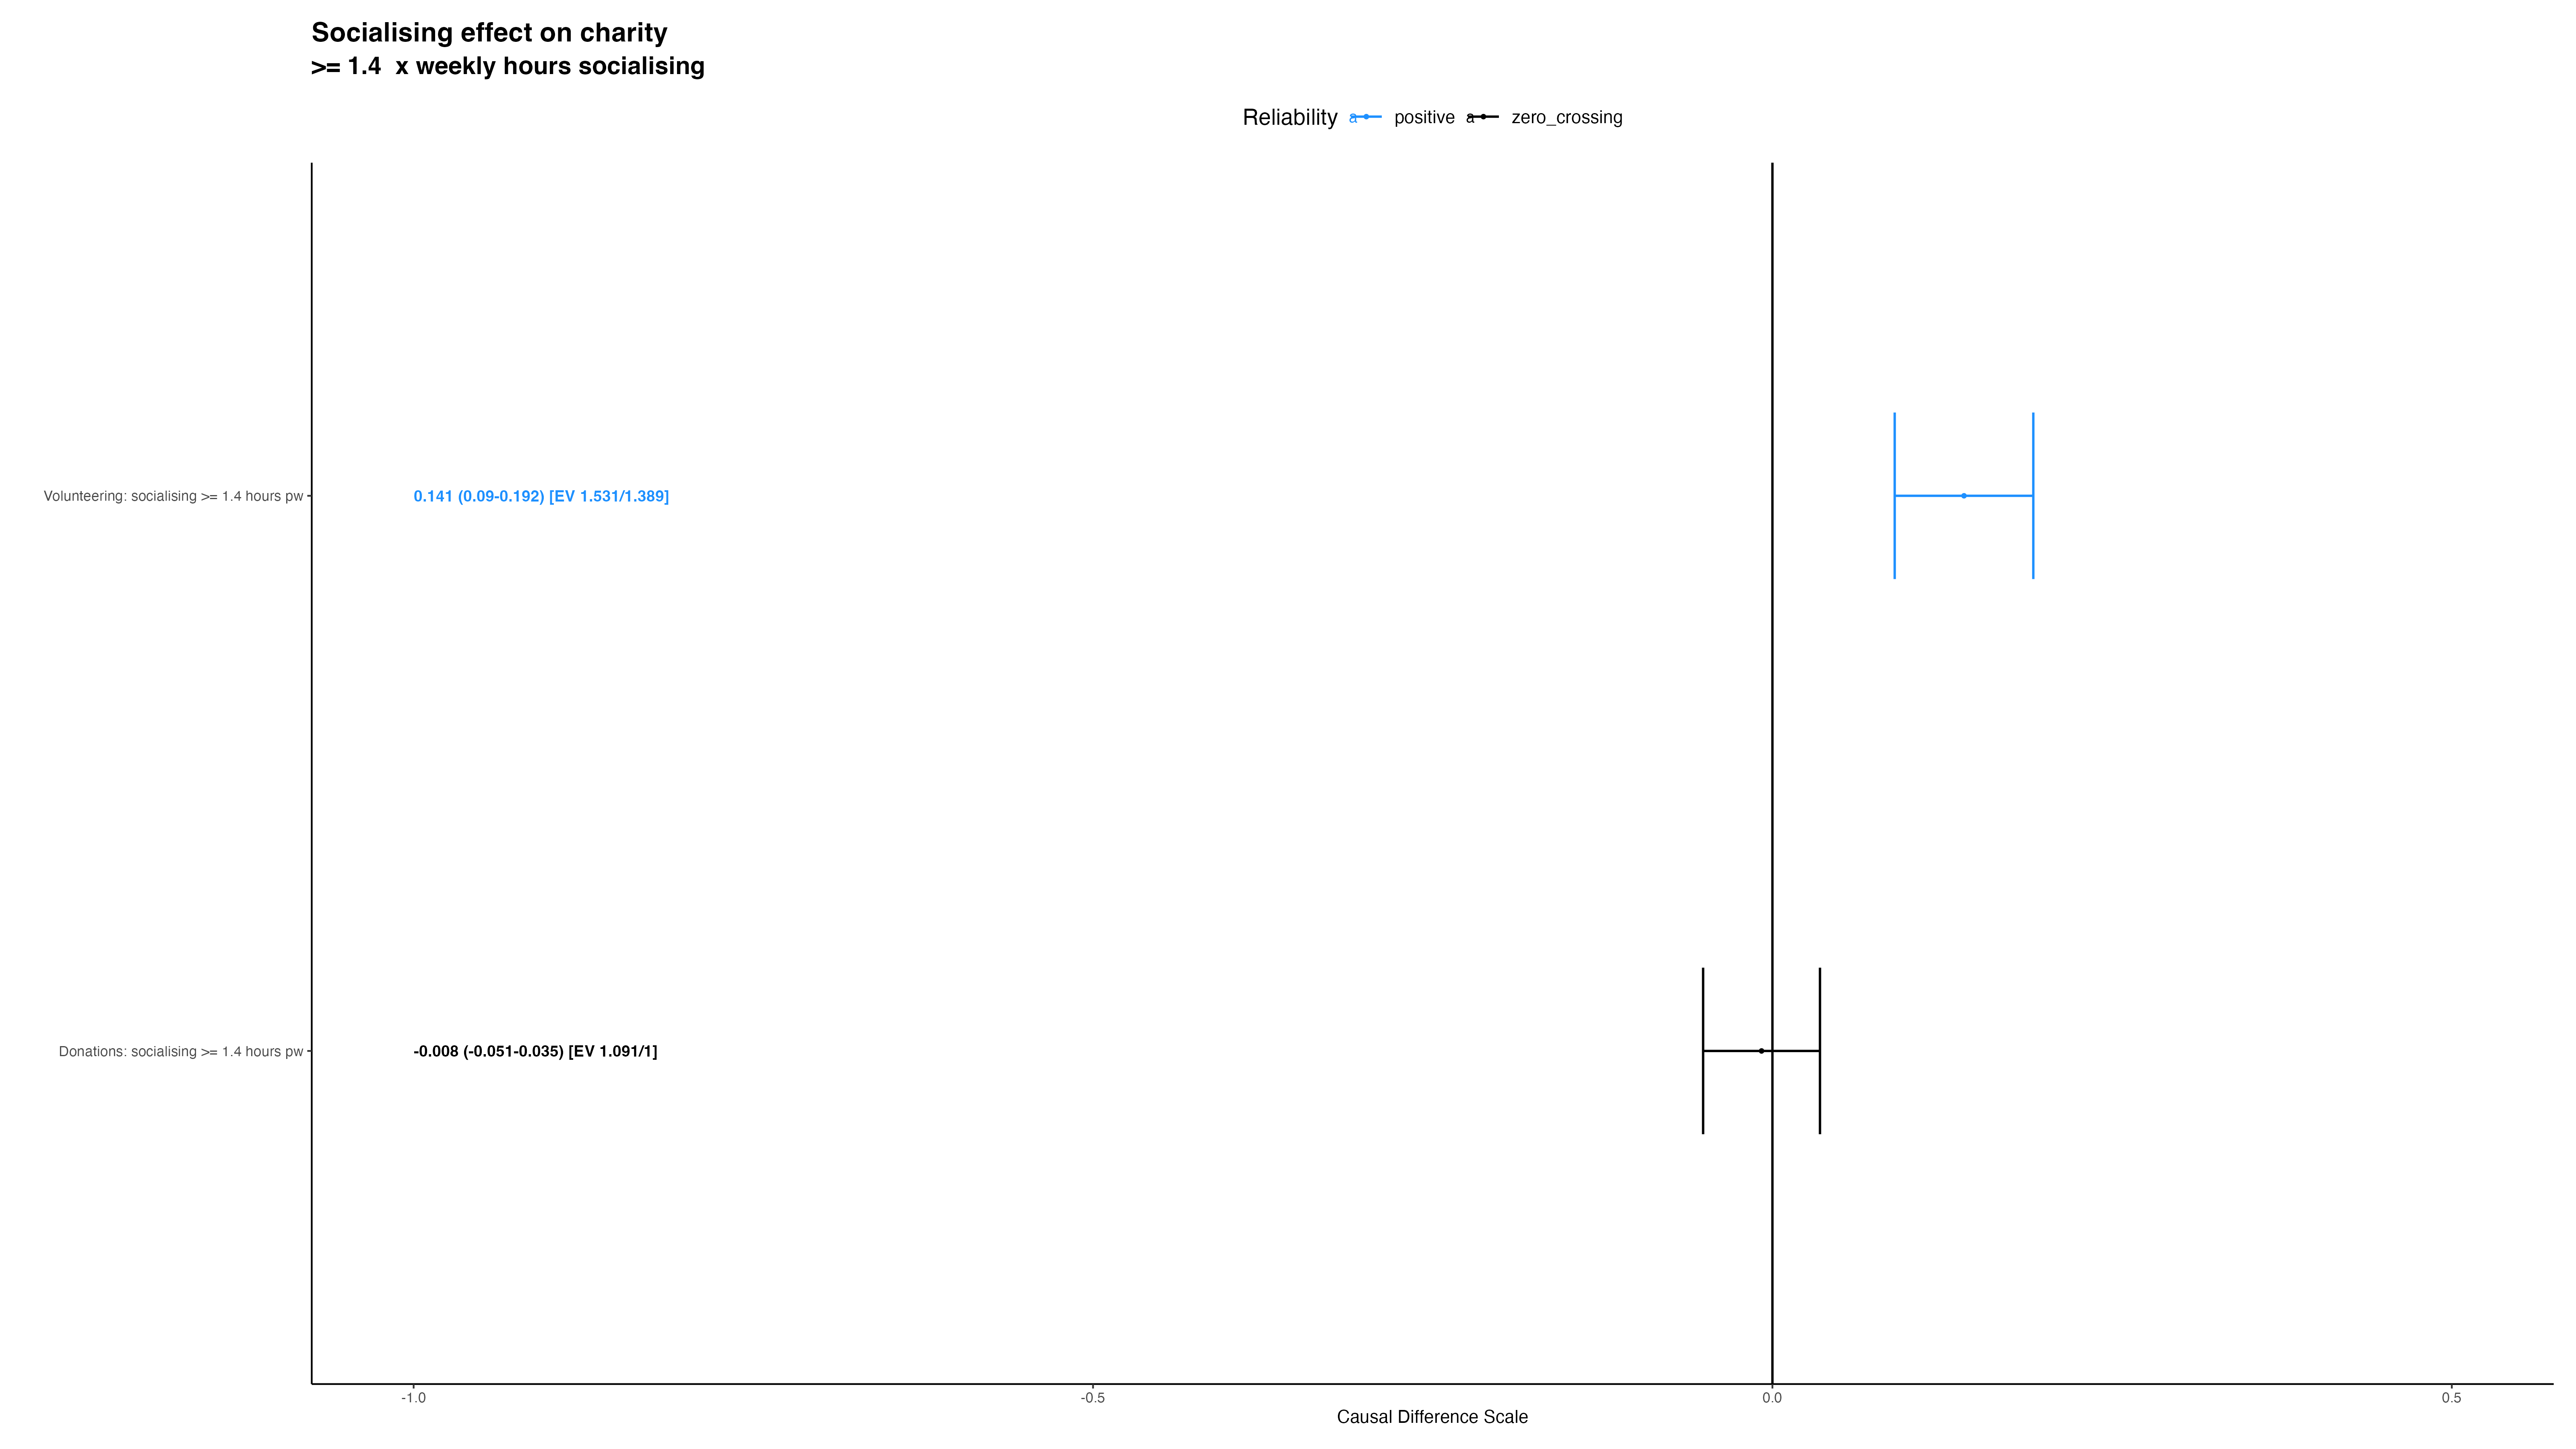
\includegraphics{plot_socializing_prosocial.png}

}

\caption{plot\_socializing\_prosocial}

\end{figure}%
\end{frame}

\begin{frame}
\begin{figure}[H]

{\centering 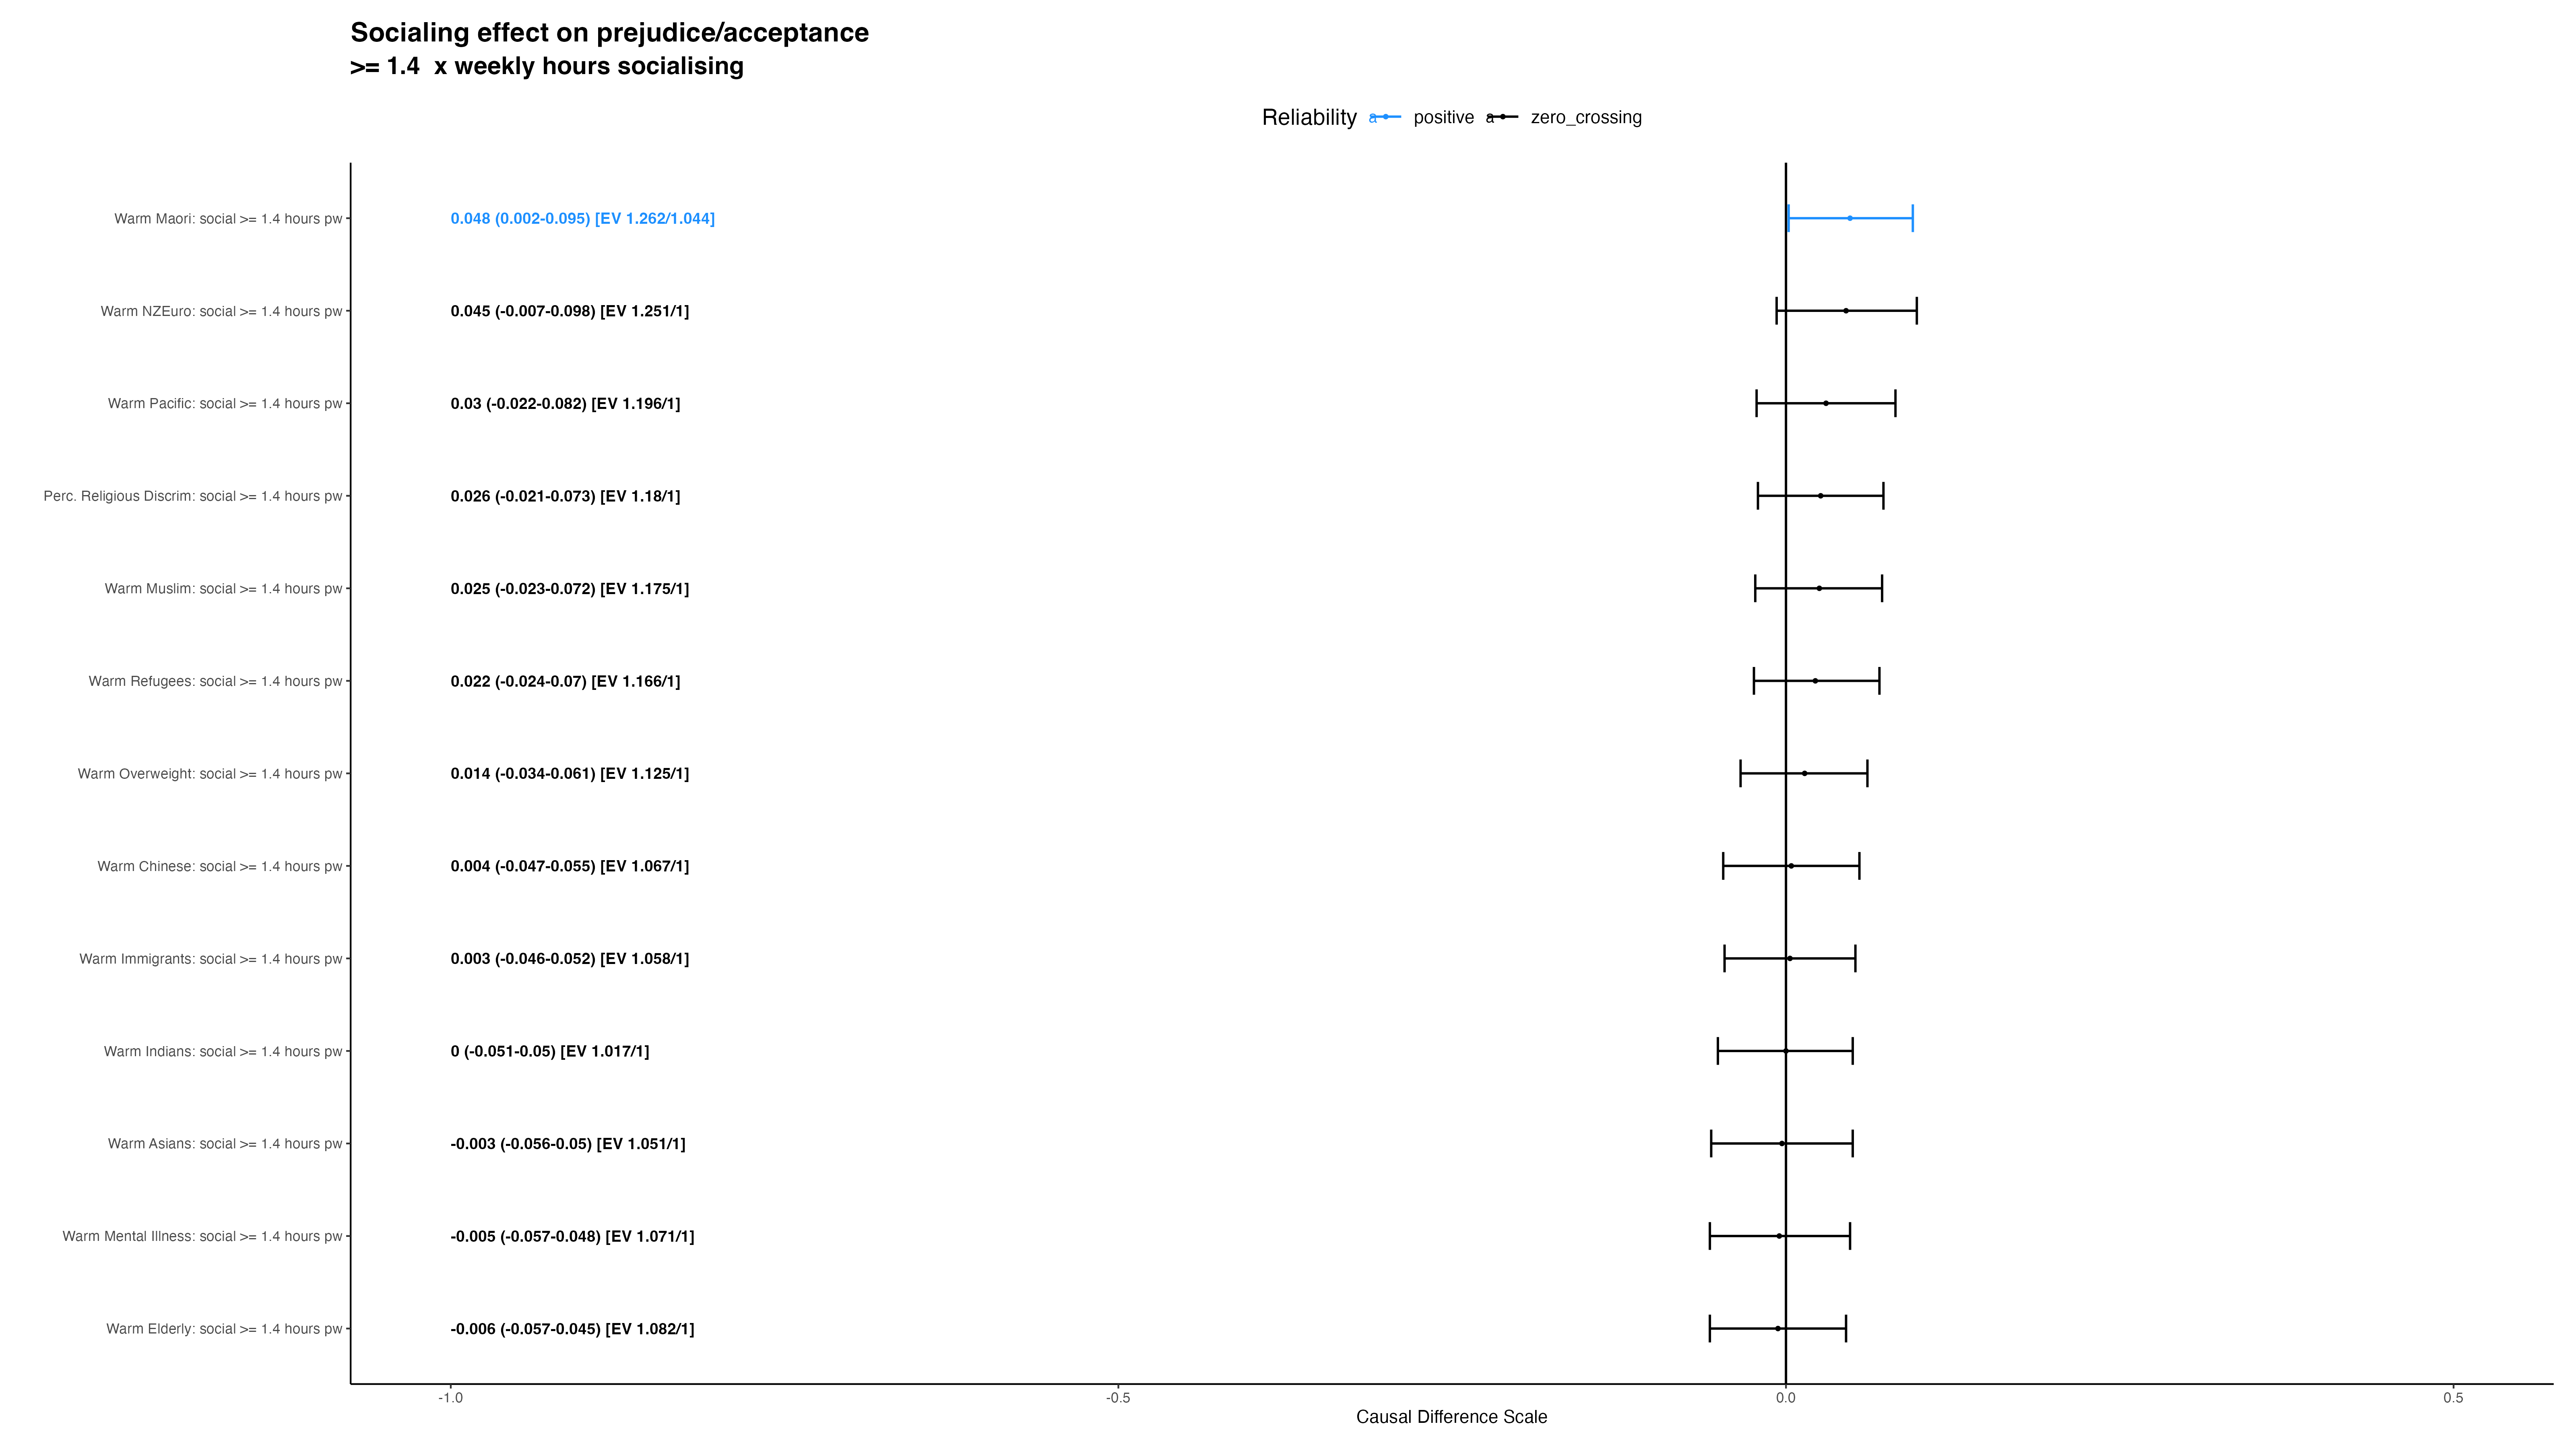
\includegraphics{plot_warm_socialising.png}

}

\caption{plot\_warm\_socialising}

\end{figure}%
\end{frame}

\begin{frame}
\begin{figure}[H]

{\centering 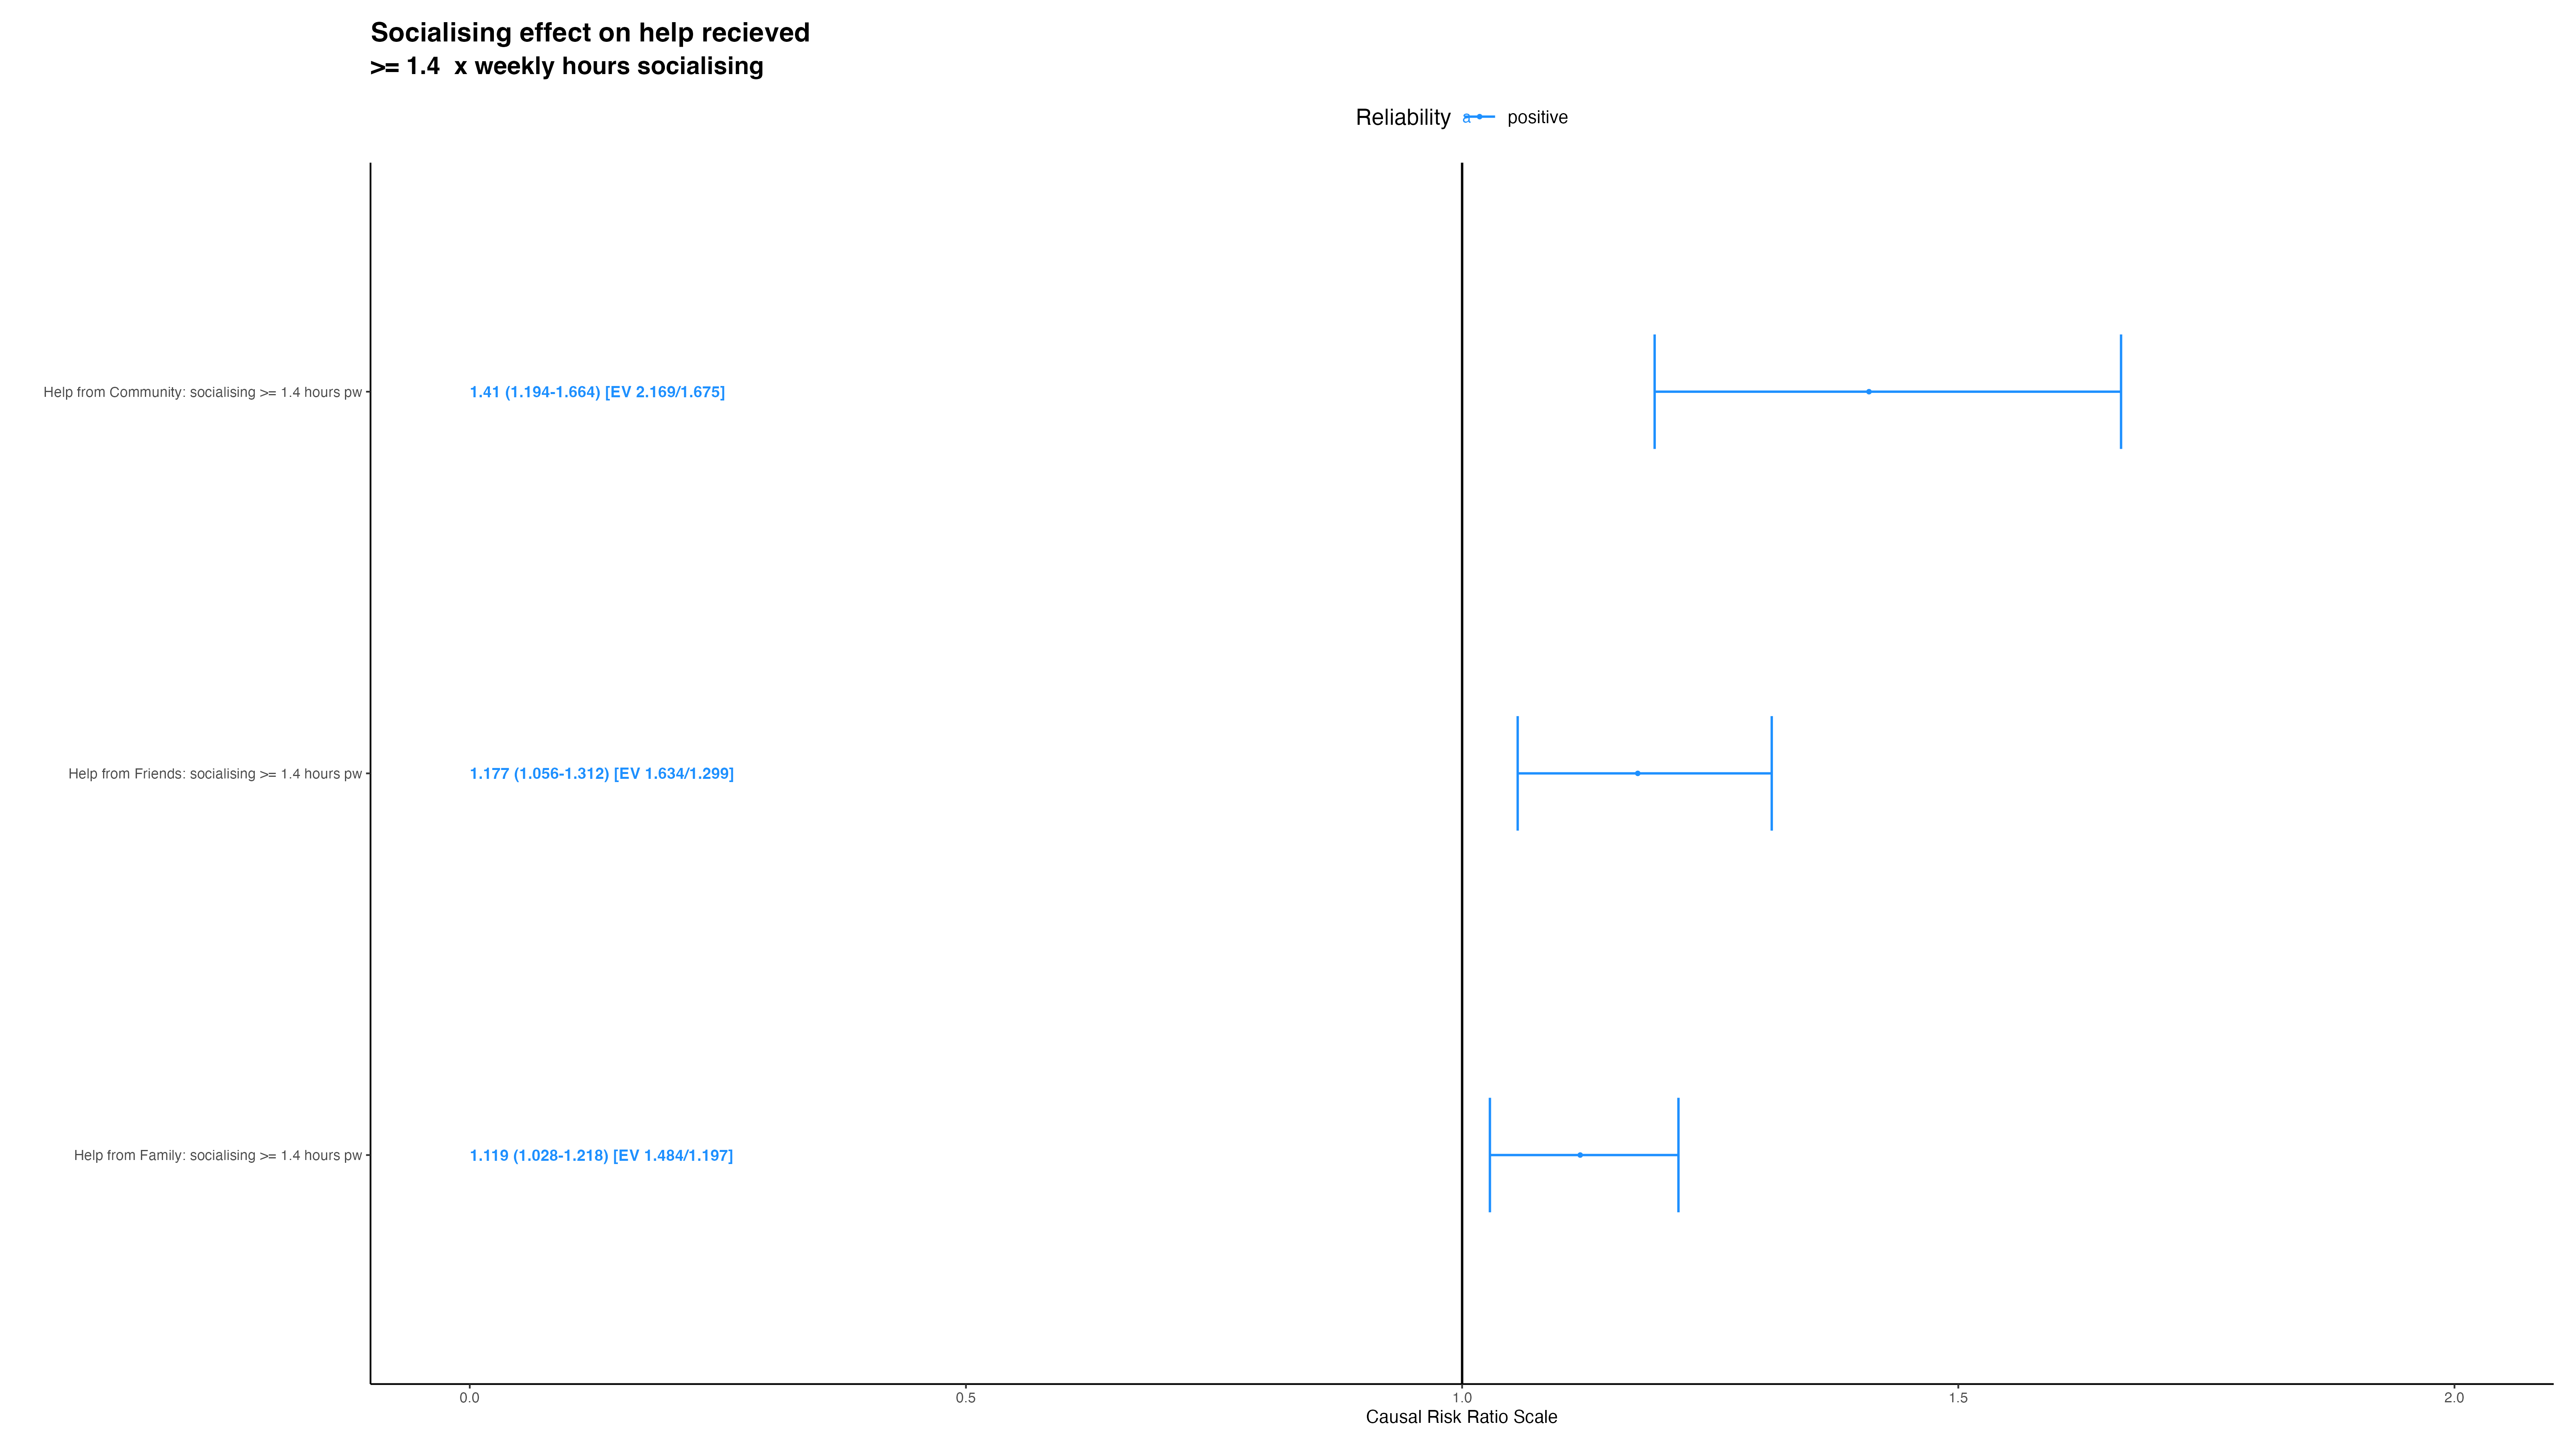
\includegraphics{plot_socialising_gain_help_received.png}

}

\caption{plot\_socialising\_gain\_help\_received}

\end{figure}%
\end{frame}

\begin{frame}{Results}
\phantomsection\label{results}
\begin{itemize}
\tightlist
\item
  Causal effects of religious service attendance on the economy are
  considerable, in expectation they represent \textasciitilde{}
  \textbf{0.048\%} of New Zealand's 2021 annual government budget.
\item
  Notably, cross-sectional associations are four times stronger, but
  these associations are \textbf{uninterpretable}
\item
  Results underscore the importance of investigating gradual cultural
  change.
\end{itemize}
\end{frame}

\begin{frame}{Summary}
\phantomsection\label{summary}
\begin{enumerate}[<+->]
\tightlist
\item
  To move beyond association to causality requires time, literally.
\item
  Big events \(\neq\) big effect sizes.
\item
  Long-term effects unclear.
\item
  Long-term change might be more important for planning.
\end{enumerate}
\end{frame}

\begin{frame}{Thanks}
\phantomsection\label{thanks}
\begin{itemize}
\tightlist
\item
  Chris G. Sibley (NZAVS lead Investigator)
\item
  Templeton Religion Trust Grant 0418
\item
  Max Planck Institute for Evolutionary Anthropology: Department
  Linguistic and Cultural Evolution
\item
  Victoria University
\item
  University of Canterbury
\item
  72,910 NZAVS participants
\end{itemize}
\end{frame}

\begin{frame}
\begin{figure}[H]

{\centering 
\includegraphics{NZAVS-QR.png}

}

\caption{NZAVS}

\end{figure}%
\end{frame}

\begin{frame}
\begin{figure}[H]

{\centering 
\includegraphics{qr-causal-diagrams.png}

}

\caption{Causal Diagrams}

\end{figure}%
\end{frame}

\begin{frame}{Extra Slides}
\phantomsection\label{extra-slides}
\end{frame}

\begin{frame}{Longitudinal Data Bring Their Own Problems}
\phantomsection\label{longitudinal-data-bring-their-own-problems}
\end{frame}

\begin{frame}{Timing of Confounder}
\phantomsection\label{timing-of-confounder}
\[ 
\threeBshortTHREEWAVE 
\]
\end{frame}

\begin{frame}{Timing of Mediator}
\phantomsection\label{timing-of-mediator}
\[
\threeCshortTHREEWAVE
\]
\end{frame}

\begin{frame}{Treatment Confounder Bias}
\phantomsection\label{treatment-confounder-bias}
\[\feedback\]
\end{frame}

\begin{frame}{Treatment Confounder Feedback}
\phantomsection\label{treatment-confounder-feedback}
\[\feedbackA\]
\end{frame}

\begin{frame}{Treatment Confounder Feedback Variation}
\phantomsection\label{treatment-confounder-feedback-variation}
\[\feedbackBshort\]
\end{frame}

\begin{frame}{Mediation}
\phantomsection\label{mediation}
\end{frame}

\begin{frame}{Total Effect}
\phantomsection\label{total-effect}
\begin{columns}[T]
\begin{column}{0.5\textwidth}
\[
TE = \mathbb{E}[Y(1)] - \mathbb{E}[Y(0)]
\]
\end{column}

\begin{column}{0.6\textwidth}
\[~~\]
\end{column}
\end{columns}
\end{frame}

\begin{frame}{Total Effect Considering Mediator}
\phantomsection\label{total-effect-considering-mediator}
\begin{columns}[T]
\begin{column}{0.5\textwidth}
\[
TE = \mathbb{E}[Y(1)] - \mathbb{E}[Y(0)]
\]
\end{column}

\begin{column}{0.5\textwidth}
\[ 
\mathbb{E}[Y(1)] = \mathbb{E}[Y(1, M(1))]
\]
\end{column}
\end{columns}
\end{frame}

\begin{frame}{Natural Direct Effect}
\phantomsection\label{natural-direct-effect}
\textbf{Natural Direct Effect (NDE)} is the effect of the treatment on
the outcome while maintaining the mediator at the level it would have
been if the treatment had \emph{not} been applied:

\[
 NDE = \textcolor{blue}{\mathbb{E}[Y(1, M(0))]} - \mathbb{E}[Y(0, M(0))]
\]
\end{frame}

\begin{frame}{Natural Indirect Effect}
\phantomsection\label{natural-indirect-effect}
\textbf{Natural Indirect Effect (NIE):} is the effect of the exposure on
the outcome that is mediated. To obtain these quantities we must compare
the potential outcome \(Y\) under treatment, where the mediator assumes
its natural level under treatment with the potential outcome when the
mediator assumes its natural value under no treatment is given:

\[
 NIE = \mathbb{E}[Y(1, M(1))] - \textcolor{blue}{\mathbb{E}[Y(1, M(0))]}
\]
\end{frame}

\begin{frame}{Decomposition}
\phantomsection\label{decomposition}
\[
\scriptsize{ \text{Total Effect (TE)} = \underbrace{\bigg\{\mathbb{E}[Y(1, M(1))] - \textcolor{blue}{\mathbb{E}[Y(1, M(0))]}\bigg\}}_{\text{Natural Indirect Effect (NIE)}} + \underbrace{\bigg\{\textcolor{blue}{\mathbb{E}[Y(1, M(0))]} - \mathbb{E}[Y(0, M(0))]\bigg\}}_{\text{Natural Direct Effect (NDE)}}}
\]
\end{frame}

\begin{frame}{Why Mediation is Difficult}
\phantomsection\label{why-mediation-is-difficult}
\[
\mediationfull
\]
\end{frame}

\begin{frame}{Interaction}
\phantomsection\label{interaction}
\end{frame}

\begin{frame}{Interaction: simplifies to}
\phantomsection\label{interaction-simplifies-to}
\[\scriptsize{\underbrace{\mathbb{E}[Y(1,1)]}_{\text{joint exposure}} - \underbrace{\mathbb{E}[Y(1,0)]}_{\text{only A exposed}} - \underbrace{\mathbb{E}[Y(0,1)]}_{\text{only B exposed}} + \underbrace{\mathbb{E}[Y(0,0)]}_{\text{neither exposed}} \neq 0} \]
\end{frame}

\begin{frame}{Key}
\phantomsection\label{key}
\[\terminologylocalconventions\]
\end{frame}

\begin{frame}
\begin{adjustbox}{height=0.5\textheight, keepaspectratio}
$$
\footnotesize \terminologydirectedgraph
$$
\end{adjustbox}
\end{frame}



\end{document}
